% ---- ETD Document Class and Useful Packages ---- %
\documentclass{ucetd}
\usepackage{subfigure,epsfig,amsfonts}
\usepackage{natbib}
\usepackage{amsmath}
\usepackage{amssymb}
\usepackage{amsthm}

\usepackage{url}


%% Use these commands to set biographic information for the title page:
\title{Stochastic computation in recurrent networks of spiking neurons}
\author{Clayton W. Seitz}
\department{Graduate Program in Biophysics}
\division{Physical and Biological Sciences}
\degree{Master of Science}
\date{Winter 2021}

%% Use these commands to set a dedication and epigraph text

\epigraph{Epigraph}

\begin{document}
%% Basic setup commands
% If you don't want a title page comment out the next line and uncomment the line after it:
\maketitle
%\omittitle

% These lines can be commented out to disable the copyright/dedication/epigraph pages
\makecopyright
%\makededication
\makeepigraph


%% Make the various tables of contents
\tableofcontents
%\listoffigures
%\listoftables

\acknowledgments
% Enter Acknowledgements here

\abstract

One of the most challenging questions in modern neuroscience is the mechanisms by which primate cortical circuits learn from example and perform inference based upon their past experience. The cerebral cortex is responsible for many higher-order brain functions including memory and . The search for principles of neural computation common to these phenomena is made extremely difficult by the diversity of cortical structures and their putative functions. Nevertheless, progress has been made in our understanding of the interplay between the organization of cortical neurons, network dynamics, and the resulting reorganization via synaptic plasticity during learning. Many deficiencies in our models of these processes can be attributed to our lack of a mathematical understanding of both the fundamental computational paradigm implemented by neural circuits and the roles of synaptic plasticity mechanisms observed \emph{in vivo}. These problems are further aggravated by the apparent stochastic features of the firing activity of neurons and experimentally observed trial-to-trial variability in population recordings. However, there is, in principle, a very powerful framework for stochastic computation evident in the Boltzmann machine: probabilistic inference by sampling. Here, we implement a recurrent spiking neural network (RSNN) as a variant of the Boltzmann machine and propose a precise mathematical role for a set of synaptic plasticity mechanisms in the formation of a set of synaptic weights that successfully ``embody" a Gaussian input statistic.


\mainmatter

\chapter{Introduction}

Recent decades have yielded a number of experimental and theoretical advances in our understanding of learning in biological neural networks through the introduction of as homosynaptic, heterosynaptic, and homeostatic plasticity. However, the precise mathematical relationship between the synaptic plasticity mechanisms or \emph{learning rules} implemented by neurons and the formation of probabilistic models of their inputs, remains elusive.

Neural network models date back to McCulloch and Pitts [1] followed later by the Hopfield network [2] which spawned an entire field of research applying techniques from the statistical physics of spin glasses to the description of neural activity. By simplifying a network of neurons firing action potentials to an ensemble of coupled spins $\sigma \in \{-1, +1\}$, the Hopfield model related the patterns learned by a network to the energy landscape over the discrete space of states. The storage capacity of these networks and the geometry of this energy landscape were of particular interest and rigorous mathematical treatment has been used to show limits on the basins of attraction in such energy landscapes [4,10,11]. However, recent experimental evidence has suggested that networks of neurons may follow a stochastic, rather than deterministic, computational paradigm. There are many examples in the literature of trial-to-trial variability in the response of cortical neurons to identical stimuli, suggesting that computations in the brain are inherently stochastic. The origins of this stochasticity are hypothesized to originate in noise in synaptic conductances and infidelity in processes clearing neurotransmitters from the synaptic cleft. Interestingly, an extension of the Hopfield model - the Boltzmann machine actually leverages stochastic activity of Ising spins to perform powerful computations [14]. In such a model, the set of synaptic weights $\Phi$ ``embody" the joint distribution $P_{\Phi}(X,R) = P_{\Phi}(X)P_{\Phi}(R|X)$ over network inputs and network response, respectively. Then, computations can be viewed as probabilistic inference after suitable transformations of the weights $\Delta\Phi$. Such physically inspired models have proven useful; however, the models are sufficiently abstract to make experimental comparisons difficult. More recent endeavors appear to make useful predictions on network dynamics by using Fokker-Planck equations to compute distributions of the membrane voltage as a function of time [5]. Here, we apply a similar formalism to the description of network dynamics with heterogeneous and stochastic synaptic weights to probe the distribution over network states $P_{\Phi}(R)$ and describe how this framework can be used to provide insights on how the neural networks embody the distribution $P_{\Phi}(R|X)$ in statistical inference tasks. To conclude, we discuss the effect of synaptic plasticity.

By solving the Fokker-Planck equations numerically for the time evolution of the distribution over membrane voltages $P_{\Phi}(V,t)$ simulataneously permits knowledge of the distribution $P_{\Phi}(\mathbf{z},t)$. To see this, consider thresholding a sample from the joint distribution $\mathbf{z} \sim \Theta\left(\mathbf{v}\right)$ where $\mathbf{v} \sim (P_{\Phi}(V,t))^{N}$. We might then ask how local synaptic plasticity rules permit the formation of cell assemblies which collectively encode stimuli.

\chapter{Statistical mechanics of a population of neurons}

In this section we make use of Fokker-Planck equations from statistical mechanics in the description of neural dynamics. A natural example is to describe the voltage dynamics of a single leaky integrate and fire (LIF) neuron that receives $N$ feedforward Poisson input spike trains. The formalism presented can then be generalized to a population of LIF neurons.\\

\section{Formalism}

We consider two main populations of neurons: an external population and a recurrent population. The input neurons are described only by their spiking activity and are symbolized by the binary vector $\mathbf{s}(t)\in \mathbb{F}_{2}^{n}$. Furthermore, we describe the \emph{state} variables of the recurrent population by a vector of voltages $\mathbf{v}(t)\in \mathbb{R}^{n\times 1}$ and a vector of so-called observable states denoted by $\mathbf{z}(t) = \Theta(\mathbf{v}(t))$ where $\Theta(v(t)) = H(v(t) - \theta)$ and $H$ is the Heaviside step function. Input neurons communicate to the recurrent population through excitatory connections summarized by the input weight matrix $\mathbf{X}\in \mathbb{R}^{n\times m}$. Similarly, a recurrent weight matrix $\mathbf{J}\in \mathbb{R}^{n\times n}$ specifies the recurrent network connectivity. The matrix $\mathbf{J}$ may contain both excitatory and inhibitory connections. Therefore, it will prove useful to partition $\mathbf{X}$ and $\mathbf{J}$ into four quadrants as follows

\begin{align}
\mathbf{X} = \begin{bmatrix}
    X_{E}\\
    X_{I} 
\end{bmatrix}  && \mathbf{J} = \begin{bmatrix}
    J_{EE} & J_{IE} \\
    J_{EI} & J_{II} 
\end{bmatrix} 
\end{align}

and an appropriate partitioning scheme is applied to the network state variables

\begin{align}
\mathbf{v} = \begin{bmatrix}
    v_{E}\\
    v_{I} 
\end{bmatrix}  && \mathbf{z} = \begin{bmatrix}
    z_{E}\\
    z_{I} 
\end{bmatrix} 
\end{align}

which are defined such that, for example, the inputs from the external and recurrent population to an excitatory neuron $j \in \{1, 2, ..., n'-1, n'\}$ with $n' \leq n$ is simply $\xi_{j}(t) = J_{EE}z_{E} + J_{IE}z_{I}$. More generally, the voltage state variable for an arbitrary neuron evolves according to the following differential equation for the voltage

\begin{equation}
\tau\dot{V}_{i} = -V_{i}(t) + \eta_{i}(t)
\end{equation}

where $\eta_{i}(t)$ is a noise term representing the total synaptic current arriving at the soma and $\dot{V}_{i}$ denotes the time derivative of $V_{i}$.  In general, we cannot predict any particular trajectory $V_{i}(t)$, and we must search for an expression for the time-dependent distribution $P(V_{i}, t)$ accounting for the sampled noise $\eta_{i}(t)$.

\section{Stochastic systems and Fokker-Planck equations}

The quantitative discussion of the dynamics of many complex systems (systems where the number of interacting units $N$ is large) in nature from networks of spiking neurons, geophysical systems, to excitable media, all necessarily require a statistical description. Indeed, enumerating the available states to such a system itself has proven intractable, even for small systems over short time scales. As an example, consider the states of an interacting system of $N$ binary variables denoted $\{z_{i}\}_{i=1}^{N}$ which might be physically realized as an ensemble of spins in a ferromagnet. Even for extremely small cases such as $N=100$ the system can take on $2^{100} = 1.26\times 10^{30}$ different configurations and by $N=300$ the number of configurations exceed our best estimates for the number of atoms in the known universe. At the same time, we cannot hope to make enough measurements of such a system to estimate the probability distribution over the space of states and make inferences on the organization and interactions of the individual elements based on such a distribution. We can, however, develop model distributions over the available states based on stochastic interaction between the individual units that account for the degrees of freedom which we cannot approach analytically - a technique often employed in the description of the statistical physics of particles. This family of techniques, often formally referred to as Langevin dynamics, is defined by the use of stochastic differential equations to model the evolution of systems with high degrees of freedom. A Fokker-Planck equation allows us to solve for the time evolution of the probability distribution over such a variable, providing insights into the dynamics which cannot be seen from any one trajectory through the space of states. 

In the context of neuroscience, the Fokker-Planck approach has been taken by many in describing the dynamics of the membrane potential distribution in a population of neurons. In the following paragraphs, we will sketch a derivation of the Fokker-Planck equation for a general stochastic process in one dimension and apply this result to networks of integrate and fire neurons.

\subsection{The Kramers-Moyal expansion}

Given many instantiations of a stochastic variable $V$, we can construct a normalize histogram over all observations as a function of time $P(V,t)$. However, in order to systematically explore the relationship between the parameterization of the process and $P(V,t)$ we require an expression for $\dot{P}(V,t)$. If we make a fundamental assumption that the evolution of $P(V,t)$ follows a Markov process i.e. its evolution has the memoryless property, then we can write

\begin{equation}
P(V, t) = \int T(V', t | V, t-\tau)P(V, t-\tau)dV
\end{equation} 

which is known at the Chapman-Kolmogorov equation. The factor $T(V', t | V, t-\tau)$ is known as the \emph{transition operator} in a Markov process and determines the evolution of $P(V,t)$ in time. We proceed by writing $T(V', t | V, t-\tau)$ in a form referred to as the Kramers-Moyal expansion

\begin{align*}
T(V', t | V, t-\tau) &= \int \delta(u-V')T(u, t | V, t-\tau)du\\
&= \int \delta(V+u-V'-V)T(u, t | V, t-\tau)du\\
\end{align*} 

If we use the Taylor expansion of the $\delta$-function 

\begin{equation*}
\delta(V+u-V'-V) = \sum_{n=0}^{\infty} \frac{(u-V)^{n}}{n!}\left(-\frac{\partial}{\partial V}\right)^{n}\delta(V-V')
\end{equation*}

Inserting this into the result from above, pulling out terms independent of $u$ and swapping the order of the sum and integration gives

\begin{align}
T(V', t | V, t-\tau) &= \sum_{n=0}^{\infty} \frac{1}{n!}\left(-\frac{\partial}{\partial V}\right)^{n}\delta(V-V')\int(u-V)^{n}T(u, t | V, t-\tau)du\\
&= \sum_{n=0}^{\infty} \frac{1}{n!}\left(-\frac{\partial}{\partial V}\right)^{n}\delta(V-V')M_{n}(V,t)
\end{align} 

noticing that $M_{n}(V,t) = \int(u-V)^{n}T(u, t | V, t-\tau)du$ is just the $n$th moment of the transition operator $T$. Plugging (2.6) back in to (2.4) gives 

\begin{align}
P(V, t) &= \int \left(1 + \sum_{n=1}^{\infty} \frac{1}{n!}\left(-\frac{\partial}{\partial V}\right)^{n} M_{n}(V,t)\right)\delta(V-V')P(V, t-\tau)dV\\
&= P(V', t-\tau) + \sum_{n=1}^{\infty} \frac{1}{n!}\left(-\frac{\partial}{\partial V}\right)^{n} \left[M_{n}(V,t)P(V,t)\right]
\end{align} 

Approximating the derivative as a finite difference and taking the limit $\tau\rightarrow 0$ gives

\begin{align}
\dot{P}(V,t)  &= \underset{\tau\rightarrow 0}{\mathrm{lim}}\left(\frac{P(V, t)-P(V, t-\tau)}{\tau}\right)\\
&= \sum_{n=1}^{\infty} \frac{1}{n!}\left(-\frac{\partial}{\partial V}\right)^{n} \left[M_{n}(V,t)P(V,t)\right]
\end{align} 

which is formally known as the Kramers-Moyal (KM) expansion. The Fokker-Planck equation is a special case of (2.10) where we neglect terms $n>2$ in the \emph{diffusion approximation}.

\subsection{Fokker-Planck for a Gaussian process}

Consider the following Langevin equation (first order stochastic differential equation) representing a leaky integration process

\begin{equation*}
\tau \dot{V}(t) = -V(t) + J\eta(t)
\end{equation*}

with initial condition $V(0) = 0$ and noise amplitude $J$. To illustrate the applicability of (2.10) in predicting the distribution $P(V,t)$, we consider the highly simplified case where the stochastic term is a 1D Gaussian white noise with linear drift and unit variance i.e. $\eta(t) \sim \mathcal{N}(\alpha t,1)$. Therefore, the first two moments are $\mu(t) = \alpha t$ and $\sigma^{2}(t) = 1$ and all higher order moments are zero, giving the following Fokker-Planck equation

\begin{align*}
\dot{P}(V,t) &= -\alpha t\frac{\partial}{\partial V}[P(V,t)] + \frac{1}{2}\frac{\partial^{2}}{\partial V^{2}}[P(V,t)]\\
\end{align*}

which we integrate numerically using the forward Euler method

\begin{align*}
P(V, t+\Delta t) &= P(V,t)+ \Delta t\left[\alpha t\cdot \frac{P(V+\Delta V, t) - P(V,t)}{\Delta V}\right] \\
&- \Delta t\left[\frac{1}{2}\frac{P(V+\Delta V, t) - 2P(V,t) + P(V-\Delta V, t)}{\Delta V^{2}}\right]
\end{align*} 

\begin{figure}
\centering
\subfigure[]{\label{fig:a}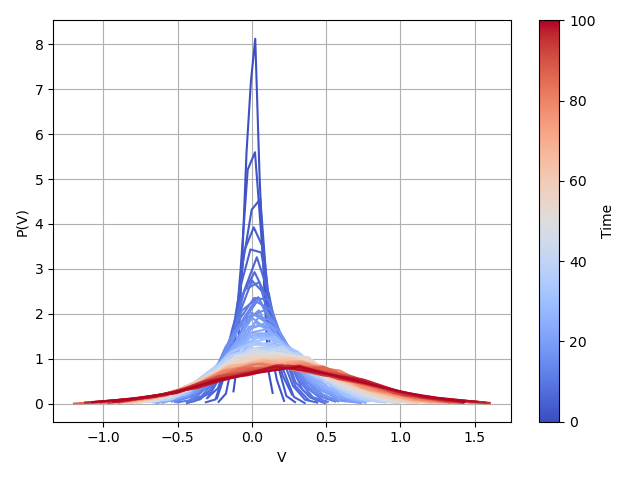
\includegraphics[width=80mm]{fig_1-A}}
\subfigure[]{\label{fig:b}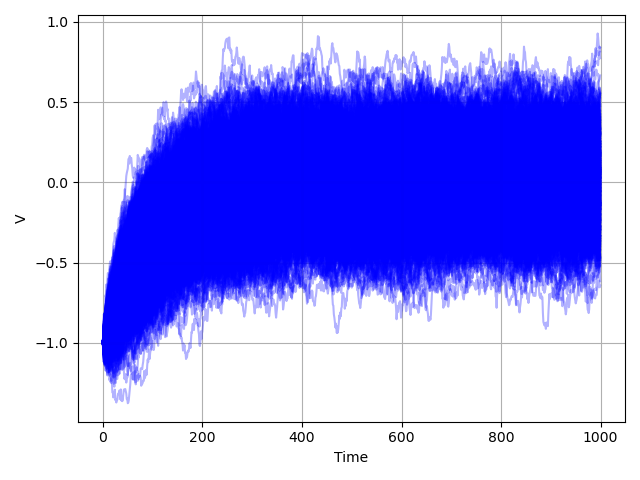
\includegraphics[width=80mm]{fig_1-B}}
\caption{Results of numerical integration of a Langevin equation for a gaussian white noise process. (a) Distribution of the stochastic variable over $N=1000$ units as a function of time. (b) Time course for $N=1000$ units}
\end{figure}


\section{Fokker-Planck for Homogeneous Sparse Networks}

The moments $M_{n}(t)$ derived above in the Kramers-Moyal expansion are dependent on the connectivity of the network and the statistics of the input. We will first consider a classic case, where we have a sparse directed network with constant synaptic efficacy between all presynaptic and postsynaptic pairs of cells. This primary pool of neurons is subject to stimulation by $N_{\mathrm{in}}$ input neurons with a connection probability $\gamma_{\mathrm{in}}$ giving $C_{\mathrm{in}} = \gamma_{\mathrm{in}}N_{\mathrm{rec}}$ unique connections between the input population and a single neuron in the recurrent pool. Within the recurrent pool, we have a connection probability of $\gamma_{\mathrm{rec}} << 1$ for any pair giving $C_{\mathrm{rec}} = \gamma_{\mathrm{rec}} N_{\mathrm{rec}}$ recurrent inputs per postsynaptic cell. We assume that a presynaptic action potential invokes a post synaptic potential (PSP) with magnitude $J_{0}$ in the postsynaptic cell with $J_{0} << \theta$ for both input and recurrent projections. The first moment of the transition operator $T(V',t| V,t-\tau)$ is given by

\begin{align*}
\mu(t) &= \mu_{in} + \mu_{rec}(t)\\
&= \left(C_{\mathrm{in}}\nu_{\mathrm{in}}(t) + C_{\mathrm{rec}}\nu_{\mathrm{rec}}(t)\right)\tau\langle J\rangle\\
&= \left(C_{\mathrm{in}}\nu_{\mathrm{in}}(t) + C_{\mathrm{rec}}\nu_{\mathrm{rec}}(t)\right)\tau J_{0}
\end{align*}

where $\nu_{\mathrm{in}}(t)$ is the rate parameter for the input Poisson process. The second moment

\begin{align*}
\sigma^{2}(t) &= \sigma_{\mathrm{rec}}^{2} + \sigma_{\mathrm{ext}}^{2}\\
&= \left(C_{\mathrm{in}}\nu_{\mathrm{in}}(t) + C_{\mathrm{rec}}\nu_{\mathrm{rec}}(t)\right)\tau\langle J^{2}\rangle\\
&= \left(C_{\mathrm{in}}\nu_{\mathrm{in}}(t) + C_{\mathrm{rec}}\nu_{\mathrm{rec}}(t)\right)\tau J_{0}^{2}
\end{align*}

After inserting the first two moments into (2.10) we arrive at the following Fokker-Planck equation

\begin{align*}
\dot{P}(V,t) &= -\frac{\partial}{\partial V}[\mu(t)P(V,t)] + \frac{1}{2}\frac{\partial^{2}}{\partial V^{2}}[\sigma^{2}(t)P(V,t)]\\
\end{align*} 

At this point, it is necessary to impose the appropriate boundary conditions on the above Fokker-Planck equation as in so as to maintain biological realism. The Fokker-Planck equation can be written as the continuity equation 

\begin{equation*}
\frac{\partial P(v,t)}{\partial t} = -\frac{\partial S}{\partial V}
\end{equation*}

(Risken, 1984) with 

\begin{equation*}
S(V,t) = -\frac{v-V_{L}-\mu}{\tau}P(V,t) - \frac{\sigma^{2}(t)}{2\tau}\frac{\partial P(V,t)}{\partial V}
\end{equation*}

which is known as the \emph{probability current} through voltage $V$ at a time $t$. The instantaneous firing rate is equivalent to the probability current through the threshold i.e. $\nu(t) = S(\theta,t)$. Furthermore, we require that the probability current through the firing threshold $P(\theta, t)=0$ and that instead this probability emerges at the resting potential after a refactory period of $\tau_{\mathrm{ref}}$. This condition gives the following boundary condition for the derivative of the probability with respect to voltage

\begin{equation*}
\frac{\partial P(\theta,t)}{\partial V} = -\frac{2\tau\nu(t)}{\sigma^{2}(t)}
\end{equation*}

To account for the refractory period $\tau_{\mathrm{ref}}$, we define an auxililary distribution

\begin{equation*}
p_{r}(t) = \int_{t-\tau_{\mathrm{ref}}}^{t} \nu(t)dt
\end{equation*}

which together with the distribution $P(V,t)$ satisfy the normalization condition:

\begin{equation*}
\int P(v,t)dV + p_{r}(t) = 1
\end{equation*}

\begin{align*}
\frac{\partial P(v,t)}{\partial t} &= \left(\mu(t) - \frac{v-v_{L}}{\tau}\right) \frac{\partial}{\partial v} P(v,t) - \frac{\sigma^{2}(t)}{2\tau}\frac{\partial^{2}}{\partial v^{2}} P(v,t) + \nu(t-\tau_{\mathrm{ref}})\delta(v-V_{R})\\
\end{align*} 


which we approximate by central finite differences

\begin{align*}
\frac{p(v, t+\Delta t) - p(v,t)}{\Delta t} &= \left(\mu(t) - \frac{v-v_{L}}{\tau}+ \mu_{ext}\right)\frac{p(v+\Delta v, t) - p(v,t)}{\Delta v} \\
&- \frac{1}{2}\left(\sigma^{2}(t) + \sigma_{ext}^{2}\right)\frac{p(v+\Delta v, t) - 2p(v,t) + p(v-\Delta v, t)}{\Delta v^{2}}
\end{align*} 


\chapter{Dynamical states of recurrent networks}
\section{Introduction}


\chapter{Stochastic computation by recurrent networks}
\section{Introduction}

\chapter{Conclusions}

% Intro to chapter one

% Format a LaTeX bibliography
\makebibliography

[1] Mculloch and Pitts. \textit{A logical calculus of the ideas imminent in nervous activity}. Journal of Mathematical Biophysics. 1943.

[2] J.J. Hopfield. \textit{Neural networks and physical systems with emergent collective computational abilities}. 1982.

[3] D.J. Amit. \textit{Spin-glass models of neural networks}. Physical Rev A. 1985.

[4] E. Gardner. \textit{The space of interactions in neural network models}. Journal of Physics A: Mathematical and General. 1988.

[5] N. Brunel. \textit{Dynamics of sparsely connected networks of excitatory and inhibitory neurons}. Journal of Computational Neuroscience. 2000. 

[6] Rosenbaum and Doiron. \textit{Balanced Networks of Spiking Neurons with Spatially Dependent Recurrent Connections}. Physical Review X. 2014.

[7] Zenke et al. \textit{Diverse synaptic plasticity mechanisms
orchestrated to form and retrieve memories
in spiking neural networks}. Nature Communications. 2015.

[8] Williams et al. \textit{Nonnegative decomposition of multivariate information}. arXiv. 2010.

[9] Amit et al. \textit{Storing infinite numbers of patterns in a spin-glass model of neural networks}. Physical Rev. Letters. 1985

[10] Nishimori. \textit{Statistical physics of spin glasses and information processing: an introduction}. Clarendon Press. 2010

[11] Buesing et al. \textit{Neural Dynamics as Sampling: A Model for Stochastic Computation in Recurrent Networks of Spiking Neurons}. PLOS Computational Biology. 2011

[12] Pecevski et al. \textit{Learning Probabilisitc Inference through Spike-Timing-Dependent Plasticitys}. eNeuro. 2016

[13] Pecevski et al. \textit{Formation and maintenance of neuronal assemblies through synaptic plasticity}. Nature Communications. 2014

[14] Pecevski et al. \textit{A learning algorithm for Boltzmann Machines}. Cognitive Science. 1985

% Figures and tables, if you decide to leave them to the end
%\input{figure}
%\input{table}

\end{document}


